\section{Spannungs- und Strommessung}
\subsection{Einleitung}
Die Messung von Spannung und Strom ist eine grundlegende Aufgabe in der Elektrotechnik. Je nach Art des Verbrauchers (hochohmig oder niederohmig) hat die Wahl der Messmethode - spannungsrichtig oder stromrichtig - einen wesentlichen Einfluss auf die Genauigkeit der Messergebnisse. Die beiden Methoden unterscheiden sich in der Art, wie Strom- und Spannungsmesser in die Schaltung eingebunden werden. Ziel dieses Versuchs ist es, die Unterschiede beider Methoden zu untersuchen und die resultierenden Widerstandswerte für verschiedene Verbraucher zu vergleichen.

\subsection{Theoretische Grundlagen}
\paragraph{Spannungsrichtige Messung}
Bei der spannungsrichtigen Messung wird der Strommesser in Reihe und der Spannungsmesser parallel zum Verbraucher geschaltet. Diese Methode ist besonders geeignet für niederohmige Verbraucher, da der Einfluss des Parallelwiderstands des Spannungsmessers vernachlässigbar ist (siehe Abbildung~\ref{subfig:K6A1a}).

\paragraph{Stromrichtige Messung}
Im Gegensatz dazu wird bei der stromrichtigen Messung der Spannungsmesser parallel zum Verbraucher und Strommesser geschaltet. Diese Methode ist ideal für hochohmige Verbraucher, da der Spannungsmesser den Stromfluss kaum beeinflusst (siehe Abbildung~\ref{subfig:K6A1b}).

\subsection{Versuchsaufbau}
Für den Versuch werden zwei unterschiedliche Verbraucherwiderstände \( R \) von \( 10\,\unit{\ohm} \) (niederohmig) und \( 1\,\unit{M\ohm} \) (hochohmig) verwendet. Die Eingangsspannung beträgt konstant \( 5\,\unit{V} \). Zwei unterschiedliche Schaltungen werden aufgebaut:
\begin{itemize}
    \item \textbf{Spannungsrichtige Messung:} Nach Abbildung~\ref{subfig:K6A1a}.
    \item \textbf{Stromrichtige Messung:} Nach Abbildung~\ref{subfig:K6A1b}.
\end{itemize}
Bei beiden Methoden werden die Spannung \( U \) und der Strom \( I \) gemessen, und der Widerstand \( R \) wird mit der Gleichung \eqref{eq:Ohm'sche Gleichung} ermittelt.

\begin{figure}[H]
    \begin{subfigure}[c]{0.5\textwidth}
        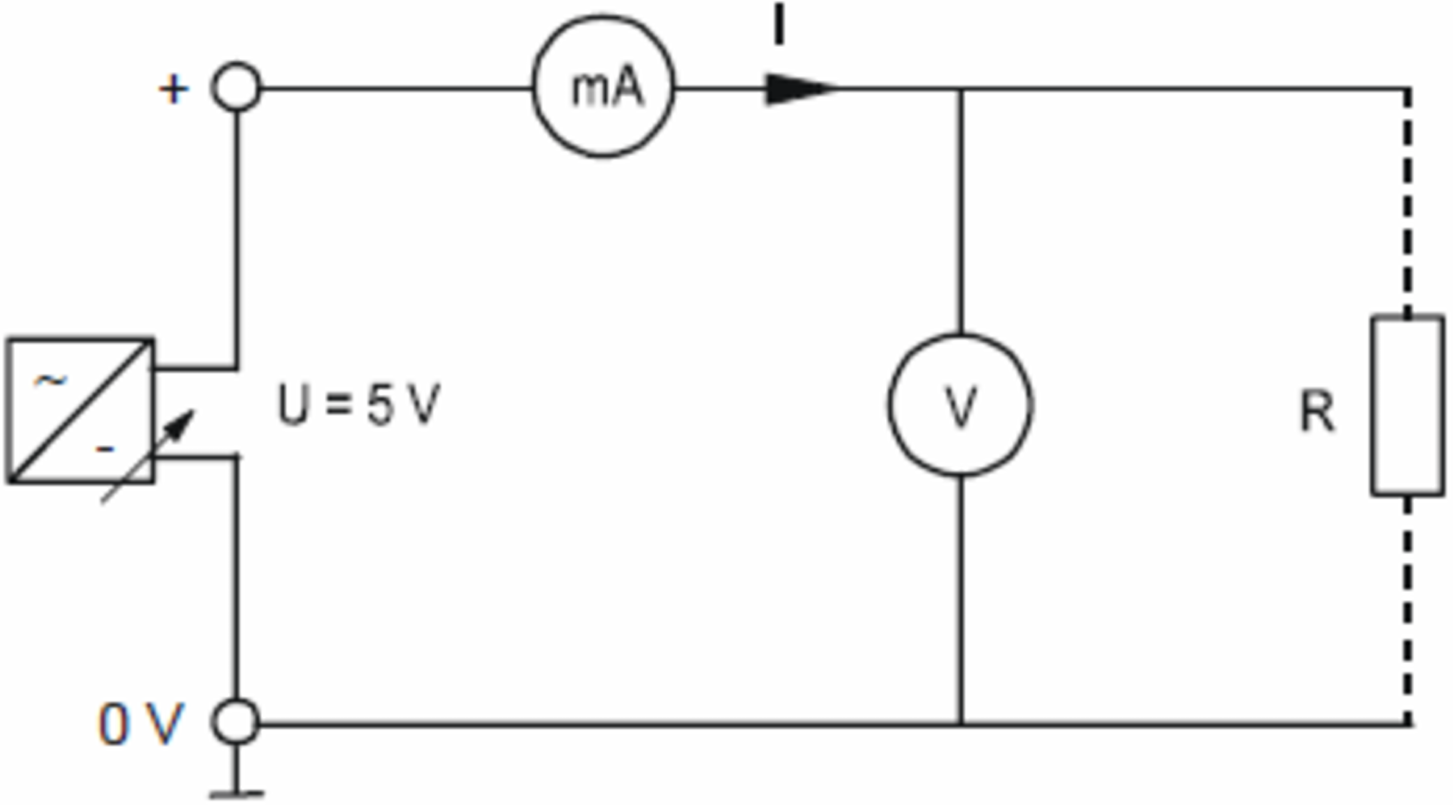
\includegraphics[width=0.95\textwidth]{Pictures/Kapitel6/Spannungsrichtig.png}
        \subcaption{Spannungsrichtige Messschaltung}
        \label{subfig:K6A1a}
    \end{subfigure}
    \begin{subfigure}[c]{0.5\textwidth}
        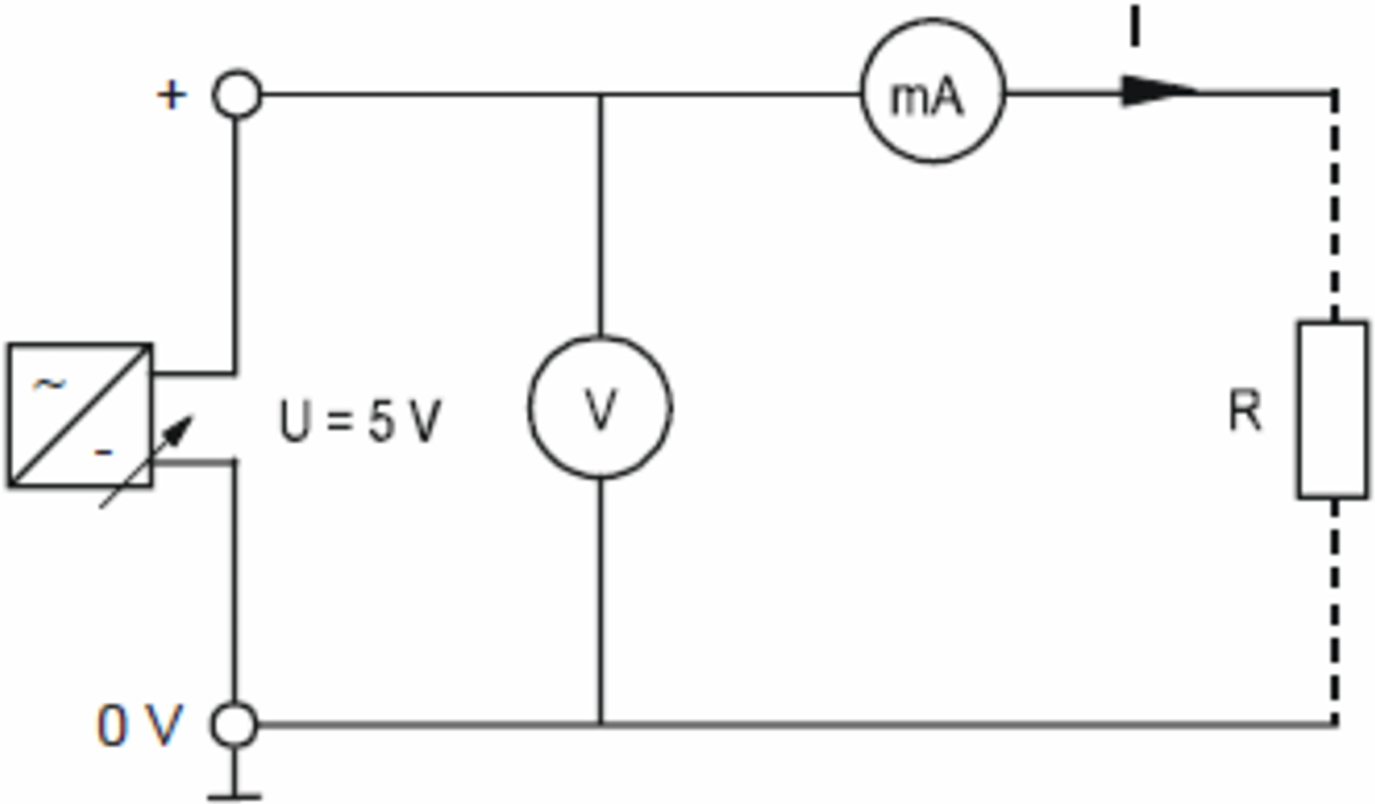
\includegraphics[width=0.9\textwidth]{Pictures/Kapitel6/Stromrichtig.png}
        \subcaption{Stromrichtige Messchaltung}
        \label{subfig:K6A1b}
    \end{subfigure}
\caption{Spannungs- und Stromrichtige Messung}
\label{fig:K6A1}
\end{figure}

\subsection{Ergebnisse}
Die Messwerte sind in den Tabellen~\ref{tab:K6T1} und~\ref{tab:K6T2} dargestellt. Sie zeigen die gemessenen und berechneten Widerstandswerte für beide Methoden.

\begin{table}[H]
\centering
\begin{footnotesize}
\caption{Ergebnisse der spannungsrichtigen Messung}
\begin{tabular}{c c c c}
\toprule
$R/\,\unit{\ohm}$ gemessen & $I/\,\unit{mA}$ & $U/\,\unit{V}$ & $R/\,\unit{\ohm}$ errechnet \\
\midrule
9,40 & 481,00 & 4,78 & 9,94 \\
\(1,0020\cdot10^6\) & 0,0054 & 4,9800 & \(0,9220 \cdot 10^6\) \\
\bottomrule
\end{tabular}
\label{tab:K6T1}
\end{footnotesize}
\end{table}

\begin{table}[H]
\centering
\begin{footnotesize}
\caption{Ergebnisse der stromrichtigen Messung}
\begin{tabular}{c c c c}
\toprule
$R/\,\unit{\ohm}$ gemessen & $I/\,\unit{mA}$ & $U/\,\unit{V}$ & $R/\,\unit{\ohm}$ errechnet \\
\midrule
9,40 & 475,00 & 4,76& 10,02 \\
\(1,0020\cdot10^6\) & 0,0048 & 4,9600  & \(1,0300 \cdot 10^6\) \\
\bottomrule
\end{tabular}
\label{tab:K6T2}
\end{footnotesize}
\end{table}

Die Abweichungen zwischen gemessenen und berechneten Werten sind jedoch nicht nur auf die Wahl der Messmethode zurückzuführen, sondern auch auf folgende Faktoren, wie Messfehler, Messungenauigkeit, Toleranz usw.

\newpage
\subsection{Diskussion und Interpretation}
Die Ergebnisse zeigen, dass die Wahl der Messmethode einen signifikanten Einfluss auf die Messgenauigkeit hat:
\begin{itemize}
    \item Spannungsrichtige Messung: Diese Methode liefert bei niederohmigen Verbrauchern zuverlässige Ergebnisse, da der Spannungsmesser den Stromfluss nicht wesentlich beeinflusst. Bei hochohmigen Verbrauchern treten jedoch deutliche Abweichungen auf, da der Spannungsmesser parallel zum hohen Widerstand eine merkliche Strombelastung erzeugt.
    \item Stromrichtige Messung: Diese Methode ist ideal für hochohmige Verbraucher, da der Strommesser den Spannungsabfall nicht signifikant beeinflusst. Bei niederohmigen Verbrauchern führt der interne Widerstand des Strommessers jedoch zu einer merklichen Spannungsreduktion.
\end{itemize}

Die richtige Wahl der Messmethode ist entscheidend für exakte Ergebnisse. Während die spannungsrichtige Messung für niederohmige Verbraucher geeignet ist, sollte bei hochohmigen Verbrauchern die stromrichtige Messung angewandt werden. Dieser Versuch verdeutlicht die praktischen Auswirkungen der Messmethoden und deren Relevanz in der Elektrotechnik.

\newpage